% followup_paper.tex -- Follow-up to the parent ARR submission.
%
% Topic: textual-gradient (TextGrad) optimisation of the parent paper's
% hand-designed Narration-of-Thought (NoT) scaffold, with a head-to-head
% comparison of two training-judge configurations (in-family vs cross-family)
% under cross-vendor adversarial evaluation.
%
% Pre-registration: Guidance_Documents/followup_study_design.md
% Raw artefacts:    divergence_study_outputs/{ng,ng2,followup}_*.{json,csv}

\documentclass[11pt]{article}

\usepackage[review]{acl}

\usepackage{times}
\usepackage{latexsym}
\usepackage[T1]{fontenc}
\usepackage[utf8]{inputenc}
\usepackage{microtype}
\usepackage{inconsolata}
\usepackage{booktabs}
\usepackage{multirow}
\usepackage{tabularx}
\usepackage{amsmath}
\usepackage{amssymb}
\usepackage{url}
\urlstyle{tt}
\usepackage{graphicx}
\usepackage{xcolor}
\usepackage{tikz}
\usetikzlibrary{positioning, arrows.meta, calc, fit, shapes.geometric, backgrounds}

% Aquatic palette mirrored from the parent paper for visual continuity.
\definecolor{stdgrey}{HTML}{7E9AAB}
\definecolor{ncotteal}{HTML}{0E7C7B}
\definecolor{ncottealdk}{HTML}{0A5C5B}
\definecolor{vendorblue}{HTML}{2E7DA0}
\definecolor{vendorsienna}{HTML}{0E5C5B}
\definecolor{vendorplum}{HTML}{5BB0A8}
\definecolor{alarmred}{HTML}{1A3B6E}
\definecolor{paleslate}{HTML}{E2EAF0}
\definecolor{paleteal}{HTML}{D9ECEB}
\definecolor{paleblue}{HTML}{D6E5EE}
\definecolor{paleplum}{HTML}{DCEEEB}
\definecolor{palealarm}{HTML}{C9D7E6}

\title{Textual-Gradient Optimisation of a Deliberative Prompt Scaffold:\\
Cross-Family Training Yields Larger Gains, Shorter Outputs,\\
and Reduces an In-Family Judge-Generosity Bias}

\author{Anonymous ARR submission}

\begin{document}
\maketitle

% ===========================================================================
\begin{abstract}
The parent ARR submission of this work introduces Narration-of-Thought (NoT), a hand-designed system prompt that reduces stakeholder collapse and uncertainty suppression on a four-generator panel.
We ask whether NoT is at or near a local optimum by applying textual-gradient descent (TextGrad) initialised at NoT under a continuous deliberative-depth loss, and run two configurations of the optimisation loop that differ only in their training judge: one in-family (training judge same vendor as training generator) and one cross-family.
Replicated against the parent paper's full four-generator panel and an adversarial cross-vendor third judge, both optimised prompts improve over the hand design on three of four generators, but the cross-family-trained prompt (NoT-v3) is strictly better than the in-family-trained prompt (NoT-v2) on every measured axis: Cliff's $\delta$ effect sizes on stakeholder count are larger or equal on all four generators, max causal hops is preserved or improved on more generators, output length is shorter ($0.59$--$0.95\times$ versus $0.82$--$1.37\times$), and the small in-family judge-generosity gap visible on the haiku generator under v2 ($0.19$ stakeholders) inverts in v3.
The takeaway: hand-designed deliberative scaffolds can be improved by textual-gradient descent, but the choice of training judge controls both the size and the cross-vendor reliability of the improvement; cross-family training is the dominant configuration on every axis we measured.
\end{abstract}

% ===========================================================================
% Hero figure: two side-by-side textual-gradient training runs (in-family
% vs cross-family), feeding a shared cross-vendor replication panel, with the
% head-to-head verdict at the bottom.
% ===========================================================================
\begin{figure*}[!t]
\centering
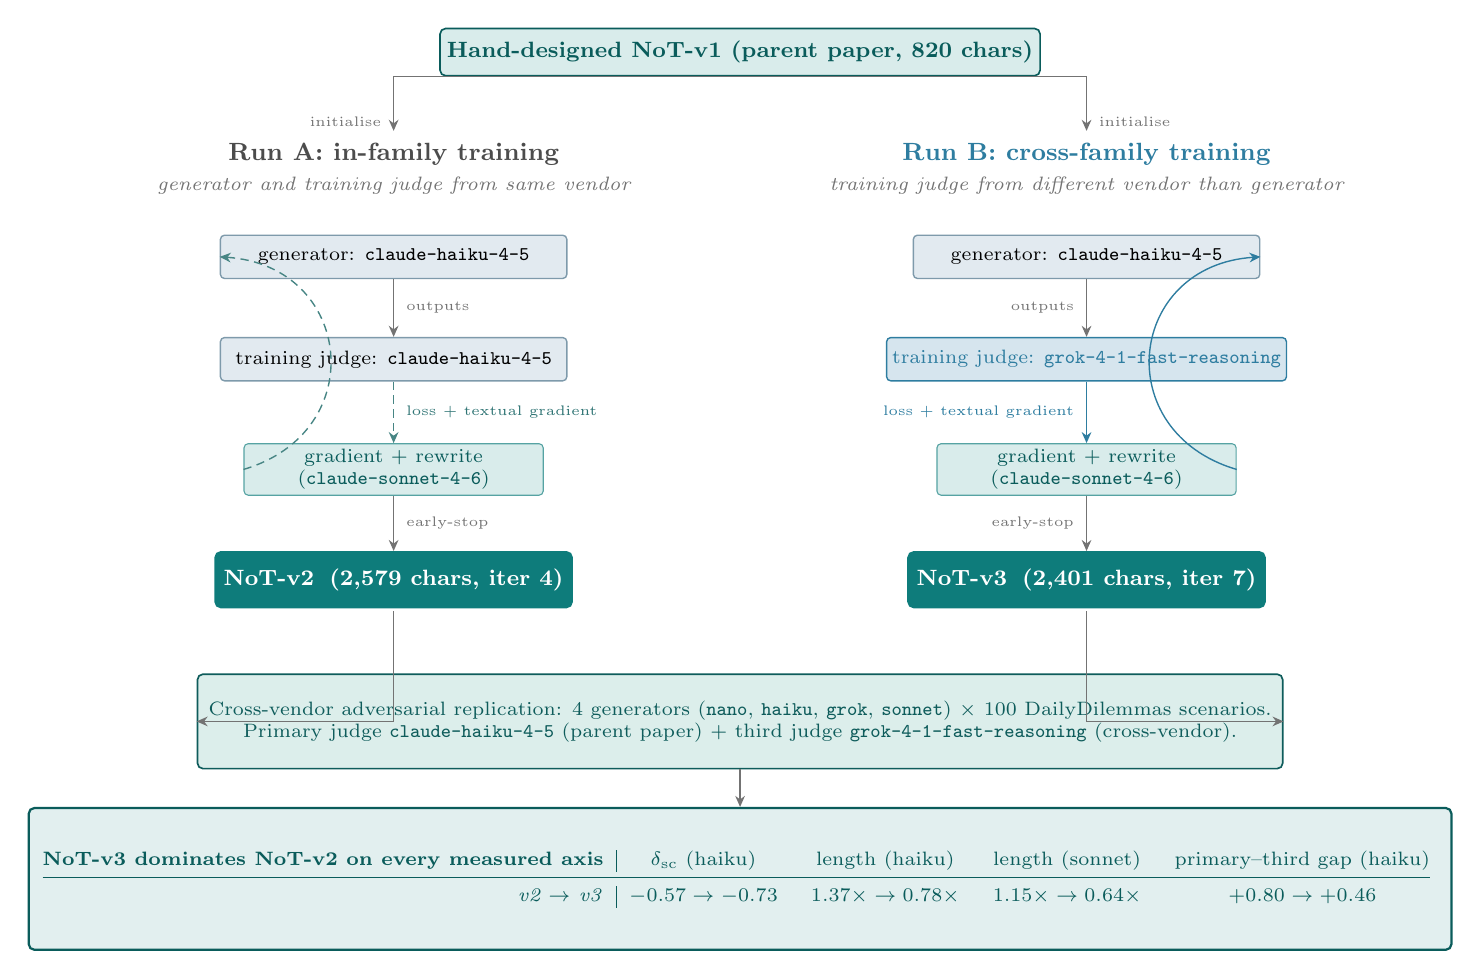
\begin{tikzpicture}[
  >={Stealth[length=4pt, width=3.5pt]},
  font=\footnotesize,
  startbox/.style={
    rectangle, draw=ncottealdk, line width=0.6pt, rounded corners=2pt,
    fill=paleteal, text=ncottealdk,
    minimum height=6mm, minimum width=42mm,
    font=\footnotesize\bfseries, align=center, inner sep=2.5pt,
  },
  genbox/.style={
    rectangle, draw=stdgrey, line width=0.5pt, rounded corners=1.5pt,
    fill=paleslate, text=black,
    minimum height=5.5mm, minimum width=44mm,
    font=\scriptsize, align=center, inner sep=2pt,
  },
  judgeinfam/.style={
    rectangle, draw=stdgrey, line width=0.5pt, rounded corners=1.5pt,
    fill=paleslate, text=black,
    minimum height=5.5mm, minimum width=44mm,
    font=\scriptsize, align=center, inner sep=2pt,
  },
  judgecross/.style={
    rectangle, draw=vendorblue, line width=0.5pt, rounded corners=1.5pt,
    fill=paleblue, text=vendorblue,
    minimum height=5.5mm, minimum width=44mm,
    font=\scriptsize, align=center, inner sep=2pt,
  },
  loop/.style={
    rectangle, draw=ncotteal!70, fill=paleteal, text=ncottealdk,
    line width=0.4pt, rounded corners=1.5pt,
    minimum height=6mm, minimum width=38mm,
    font=\scriptsize, align=center, inner sep=2pt,
  },
  outbox/.style={
    rectangle, draw=ncotteal, line width=0.8pt, rounded corners=2pt,
    fill=ncotteal, text=white,
    minimum height=7mm, minimum width=44mm,
    font=\footnotesize\bfseries, align=center, inner sep=3pt,
  },
  evalbox/.style={
    rectangle, draw=vendorsienna, line width=0.6pt, rounded corners=2pt,
    fill=paleplum, text=vendorsienna,
    minimum height=12mm, minimum width=96mm,
    font=\scriptsize, align=center, inner sep=4pt,
  },
  verdictbox/.style={
    rectangle, draw=ncottealdk, line width=0.8pt, rounded corners=2pt,
    fill=ncotteal!12, text=ncottealdk,
    minimum height=18mm, minimum width=160mm,
    font=\scriptsize, align=center, inner sep=5pt,
  },
  arr/.style={->, line width=0.45pt, color=black!55},
  arrloop/.style={->, line width=0.5pt, color=ncottealdk!75, densely dashed},
  arrcross/.style={->, line width=0.5pt, color=vendorblue},
  panelhead/.style={font=\small\bfseries, align=center},
  panelsub/.style={font=\scriptsize\itshape, align=center, text=black!55, inner sep=1pt},
]

% Shared hand-designed starting prompt
\node[startbox] (v1) at (0, 4.6) {Hand-designed NoT-v1 (parent paper, 820 chars)};

% --- Left panel: in-family training ---
\begin{scope}[shift={(-4.4, 0)}]
  \node[panelhead, text=black!70] at (0, 3.3) {Run A: in-family training};
  \node[panelsub] at (0, 2.9) {generator and training judge from same vendor};

  \node[genbox]     (gA) at (0, 2.0) {generator: \texttt{claude-haiku-4-5}};
  \node[judgeinfam] (jA) at (0, 0.7) {training judge: \texttt{claude-haiku-4-5}};
  \node[loop]       (lA) at (0,-0.7) {gradient $+$ rewrite\\(\texttt{claude-sonnet-4-6})};

  \draw[arr]     (gA.south) -- node[right=1pt, font=\tiny, text=black!55] {outputs} (jA.north);
  \draw[arrloop] (jA.south) -- node[right=1pt, font=\tiny, text=ncottealdk!85] {loss $+$ textual gradient} (lA.north);
  \draw[arrloop, bend right=80, looseness=1.6] (lA.west) to (gA.west);

  \node[outbox] (oA) at (0,-2.1) {NoT-v2\;\;(2,579 chars, iter 4)};
  \draw[arr, line width=0.5pt] (lA.south) -- node[right=1pt, font=\tiny, text=black!55] {early-stop} (oA.north);
\end{scope}

% --- Right panel: cross-family training ---
\begin{scope}[shift={(4.4, 0)}]
  \node[panelhead, text=vendorblue] at (0, 3.3) {Run B: cross-family training};
  \node[panelsub] at (0, 2.9) {training judge from different vendor than generator};

  \node[genbox]     (gB) at (0, 2.0) {generator: \texttt{claude-haiku-4-5}};
  \node[judgecross] (jB) at (0, 0.7) {training judge: \texttt{grok-4-1-fast-reasoning}};
  \node[loop]       (lB) at (0,-0.7) {gradient $+$ rewrite\\(\texttt{claude-sonnet-4-6})};

  \draw[arr]      (gB.south) -- node[left=1pt, font=\tiny, text=black!55] {outputs} (jB.north);
  \draw[arrcross] (jB.south) -- node[left=1pt, font=\tiny, text=vendorblue] {loss $+$ textual gradient} (lB.north);
  \draw[arrcross, bend left=80, looseness=1.6] (lB.east) to (gB.east);

  \node[outbox] (oB) at (0,-2.1) {NoT-v3\;\;(2,401 chars, iter 7)};
  \draw[arr, line width=0.5pt] (lB.south) -- node[left=1pt, font=\tiny, text=black!55] {early-stop} (oB.north);
\end{scope}

% v1 splits left/right to initialise both runs
\draw[arr] (v1.south) -| node[pos=0.92, left=1pt, font=\tiny, text=black!55] {initialise}
           (-4.4, 3.6);
\draw[arr] (v1.south) -| node[pos=0.92, right=1pt, font=\tiny, text=black!55] {initialise}
           ( 4.4, 3.6);

% --- Shared replication panel ---
\node[evalbox] (ev) at (0,-3.9) {
  Cross-vendor adversarial replication:
  $4$ generators (\texttt{nano}, \texttt{haiku}, \texttt{grok}, \texttt{sonnet}) $\times$ $100$ DailyDilemmas scenarios.\\
  Primary judge \texttt{claude-haiku-4-5} (parent paper) $+$ third judge \texttt{grok-4-1-fast-reasoning} (cross-vendor).
};

\draw[arr] (-4.4,-2.5) |- (ev.west);
\draw[arr] ( 4.4,-2.5) |- (ev.east);

% --- Verdict / head-to-head box ---
\node[verdictbox] (vd) at (0,-5.9) {%
  \begin{tabular}{@{}r@{\;\;}|@{\;\;}cccc@{}}
  \textbf{NoT-v3 dominates NoT-v2 on every measured axis} &
  $\delta_{\mathrm{sc}}$ (haiku) & length (haiku) & length (sonnet) & primary--third gap (haiku) \\
  \midrule
  \emph{v2 $\to$ v3} & $-0.57 \to -0.73$ & $1.37\times \to 0.78\times$ & $1.15\times \to 0.64\times$ & $+0.80 \to +0.46$ \\
  \end{tabular}
};

\draw[arr] (ev.south) -- (vd.north);

\end{tikzpicture}
\caption{Two textual-gradient training runs that differ only in the choice of training judge.
\textbf{Run A (in-family)} uses \texttt{claude-haiku-4-5} as both generator and training judge---the same vendor that the parent paper's primary judge later uses on the four-generator panel---and produces \textbf{NoT-v2}.
\textbf{Run B (cross-family)} uses \texttt{grok-4-1-fast-reasoning} (a different vendor) as the training judge and produces \textbf{NoT-v3}.
Optimiser model, dataset, training split, loss, and early-stopping criteria are identical across the two runs.
Both prompts are then replicated against the same four-generator $\times$ $100$-scenario panel, each cell scored by both the parent paper's primary judge and an adversarial cross-vendor third judge.
NoT-v3 dominates NoT-v2 on every measured axis (bottom row): equal-or-larger Cliff's $\delta$ improvements on three of four generators, shorter outputs on every generator, and a reduced in-family primary--third stakeholder-count gap on the in-family generator.}
\label{fig:hero}
\end{figure*}

% ===========================================================================
\section{Introduction}
\label{sec:intro}

Structured prompt scaffolds for ethical reasoning reduce two recurrent failure modes of single-pass chain-of-thought: \emph{stakeholder collapse} (the trace names at most one affected party) and \emph{uncertainty suppression} (the trace commits without articulating any unknown).
The parent ARR submission of this work \citep{anon24parent} introduces Narration-of-Thought (NoT), a five-section system prompt that forces the model to (1) name the decision-maker, (2) enumerate stakeholders, (3) project two-step consequences, (4) name uncertainties, and (5) only then commit.
On a four-generator panel evaluated on $100$ DailyDilemmas scenarios \citep{chiu24}, NoT cuts stakeholder collapse from up to $31\%$ to under $1\%$ and uncertainty suppression from up to $72\%$ to $1$--$24\%$.

This paper asks two questions about that hand-designed prompt:
\begin{enumerate}\setlength{\itemsep}{1pt}
\item Can automatic search over the prompt space produce a better NoT?
\item Does the choice of judge during automatic search affect whether the resulting prompt's gains survive a cross-vendor evaluator?
\end{enumerate}

We apply textual-gradient descent \citep{yuksekgonul2024textgrad}---LLM-written diagnoses of batch failures and prompt rewrites---initialised at the hand-written NoT prompt with a continuous deliberative-depth loss.
We run the optimisation loop twice with everything held identical except the training judge: once with an in-family training judge (\texttt{claude-haiku-4-5}, same vendor as the training generator) and once with a cross-family training judge (\texttt{grok-4-1-fast-reasoning}, different vendor).
We then replicate both optimised prompts across the parent paper's full four-generator panel, each scored by the original in-family primary judge and an adversarial cross-vendor third judge.
Figure~\ref{fig:hero} summarises this two-run design and the head-to-head verdict.

We find that both optimised prompts improve stakeholder coverage over NoT-v1 on three of four generators by large Cliff's $\delta$ (medium-to-large effect sizes), but the cross-family-trained prompt (NoT-v3) is strictly better than the in-family-trained prompt (NoT-v2) on every measured axis: larger raw effect sizes on three of four generators, length-residualised effects preserved, shorter outputs on every generator, no regression on the fourth generator, and a small in-family judge-generosity gap visible under v2 on the in-family generator that inverts sign under v3.
On the only generator where the third judge gives non-degenerate binary agreement scores (\texttt{grok}, where binary failure marginals are non-zero), inter-judge $\kappa$ rises from $0.57$ and $0.73$ under v2 to $0.75$ and $0.92$ under v3.

The recommendation is methodological: when textual-gradient prompt optimisation targets cross-vendor deployment, the training judge should be drawn from a different vendor than the training generator.
The cross-family configuration dominates the in-family configuration on every metric we measured, at no additional inference cost during training.

% ===========================================================================
\section{Background}
\label{sec:background}

\paragraph{Narration-of-Thought (NoT).}
The parent paper \citep{anon24parent} defines NoT as a system prompt that constrains the model's chain-of-thought to five named sections (\emph{Protagonist}, \emph{Stakeholders}, \emph{Consequences}, \emph{Uncertainty}, \emph{Decision}).
Each section instructs the model in second person what to produce.
The prompt is $820$ characters; we treat its exact wording as the initialisation for our optimisation runs and refer to it as NoT-v1.

\paragraph{Judge rubric.}
The parent paper's JSON-output rubric codes each model trace on integer-valued \emph{stakeholder count} ($\text{sc}$, distinct affected parties named), \emph{uncertainty score} ($\text{us}$, explicit unknowns or hedges named before commitment), and \emph{max causal hops} ($\text{mh}$, longest projected consequence chain).
Binary failure modes derive mechanically: \emph{stakeholder collapse} ($\text{sc} \leq 1$) and \emph{uncertainty suppression} ($\text{us} = 0$).
The same rubric is used here, applied by a primary judge (\texttt{claude-haiku-4-5}, same as the parent paper) and by an adversarial third judge (\texttt{grok-4-1-fast-reasoning}).

\paragraph{Textual-gradient descent.}
\citet{yuksekgonul2024textgrad} introduce TextGrad as a framework where prompt-level optimisation is performed by a language-model optimiser that reads the current prompt and a batch of its evaluations and writes (i) a textual gradient---a diagnosis of the prompt's shortfalls---and (ii) a rewritten prompt that addresses the gradient.
Their original work uses binary task accuracy as the loss; we adapt the framework to a continuous deliberative-primitive loss.

% ===========================================================================
\section{Method}
\label{sec:method}

\subsection{Continuous Loss}

We define a per-output cell loss
\begin{equation}
  \ell = \max(0,\, 4 - \text{sc}) + \max(0,\, 2 - \text{us}),
  \label{eq:loss}
\end{equation}
and a batch loss $L = |B|^{-1} \sum_{b \in B} \ell_b$.
The thresholds $4$ and $2$ are mid-band NoT-v1 cell values in the parent study, chosen so that the loss is non-trivial even when the binary failure modes already fire at zero.
A binary loss provides no gradient once failure rates fall below $5\%$ (as is the case for NoT-v1 on the training generator); the continuous loss reintroduces signal in this regime.

\subsection{Optimisation Loop}

\paragraph{Forward pass.}
For each prompt $p$ and a batch of $k = 10$ scenarios $B$, generate outputs $\{o_b\}$ with the target generator (\texttt{max\_tokens} $= 4096$), code each $o_b$ with the training judge to obtain $(\text{sc}_b, \text{us}_b)$, compute $L$.

\paragraph{Backward pass.}
Feed the current prompt, the batch outputs, their codes, and $L$ to an optimiser LLM (\texttt{claude-sonnet-4-6}, held constant across both runs).
The optimiser writes a textual gradient: a $4$--$8$ sentence diagnosis of which sub-instruction in the current prompt causes the observed shortfall.
It is told the prompt encodes a five-section scaffold and is free to retain, modify, rename, or drop any section.

\paragraph{Update step.}
The same optimiser LLM rewrites the prompt to address the gradient.
Constraints: $\leq 400$ words, no named ethical frameworks, five-section structure may be altered.

\paragraph{Early stopping.}
Training halts when three consecutive iterations each reduce $L$ by less than $5\%$, or after $10$ iterations.

\subsection{Two Training Regimes}

We run the optimisation loop twice with everything held identical except the training judge.

\begin{description}\setlength{\itemsep}{2pt}
\item[Run A (in-family).] Generator and training judge both \texttt{claude-haiku-4-5}; same vendor.
The training judge is the same model that the parent study's primary judge later uses on the four-generator panel.
Output prompt: \textbf{NoT-v2}.
\item[Run B (cross-family).] Generator \texttt{claude-haiku-4-5}; training judge \texttt{grok-4-1-fast-reasoning}; different vendors.
Output prompt: \textbf{NoT-v3}.
\end{description}

\noindent Optimiser model, dataset, training split (seed-43 stratified $30$-scenario subsample), held-out eval split (seed-42 indices $30$--$59$), loss, and early-stopping criteria are identical across the two runs.
Pre-registration document and per-iteration artefacts are listed in Appendix~\ref{app:repro}.

\subsection{Cross-Vendor Replication}

For each optimised prompt, we replicate against the parent paper's full four-generator panel of Experiment~1: \texttt{gpt-5.4-nano} ($N = 5$ per cell), \texttt{claude-haiku-4-5} ($N = 20$), \texttt{grok-4-1-fast-reasoning} ($N = 5$), \texttt{claude-sonnet-4-6} ($N = 5$), all on the same $100$-scenario DailyDilemmas sample.
Each v2 and v3 cell is coded by the primary judge \texttt{claude-haiku-4-5} (same as the parent paper) and re-coded by the adversarial third judge \texttt{grok-4-1-fast-reasoning}, the most cross-vendor adversarial configuration available on our three-vendor panel.\footnote{The cross-family training judge (Run B) and the cross-vendor evaluation third judge are the same model. The implication of this design constraint is discussed in Limitations.}
Inter-judge agreement on binary labels is reported as Cohen's $\kappa$ \citep{cohen60}; effect sizes are Cliff's $\delta$ \citep{cliff93} with $1000$-bootstrap $95\%$ CIs.
Total LLM-call budget: $\approx 14{,}000$ generation and judge calls per replication plus $\approx 3{,}500$ third-judge calls.

% ===========================================================================
\section{Optimised Prompts}
\label{sec:prompts}

\paragraph{NoT-v2 (in-family training).}
Run~A early-stopped after $4$ iterations.
NoT-v2 ($2{,}579$ characters) keeps the five-section scaffold but renames sections as bolded questions (\emph{Who is deciding?}, \emph{Who is affected?}\ldots) and makes two substantive additions:
(i)~the Stakeholders section gains an explicit floor (``Aim for at least five distinct stakeholders with individuated stakes'') with instructions to include indirect parties and bystanders;
(ii)~the Uncertainty section gains a per-action floor (``at least three distinct uncertainties'') with instructions to state the consequence of each unknown.
A trailing four-bullet block adds writing principles (precision over length, visible complexity, concrete stakes, consequence framing).

\paragraph{NoT-v3 (cross-family training).}
Run~B early-stopped after $7$ iterations.
NoT-v3 ($2{,}401$ characters) preserves the same five-question structure but makes three different choices:
(i)~the Stakeholders floor rises to six (``at least six distinct parties; if you find more, include them'') with instructions to consider future generations;
(ii)~the Uncertainty section is reframed per-stakeholder rather than per-action (``For every party you named and every realistic course of action you are considering, state at least one specific uncertainty\ldots No party should be skipped'');
(iii)~the closing block emphasises conciseness directly (``One sharp sentence per stakeholder stake. One precise unknown per party. Avoid restating what earlier reasoning already established'').

The two prompts converge on a higher stakeholder floor and explicit per-item uncertainty enumeration, but differ on where the uncertainty grain is attached (per-action in v2, per-stakeholder in v3) and on whether the closing block requests longer or tighter prose.
Section~\ref{sec:results} shows this difference matters: NoT-v3 produces shorter outputs than NoT-v2 on every generator while reaching equal-or-larger stakeholder-count gains.

Full verbatim text for both prompts is in Appendix~\ref{app:prompts}.

% ===========================================================================
\section{Results}
\label{sec:results}

\subsection{Head-to-Head: Primary Judge}
\label{sec:head_to_head_prim}

\begin{table*}[t]
\centering\small
\begin{tabular}{lcccccc}
\toprule
& \multicolumn{3}{c}{\textbf{NoT-v2 vs NoT-v1}} & \multicolumn{3}{c}{\textbf{NoT-v3 vs NoT-v1}} \\
\cmidrule(lr){2-4}\cmidrule(lr){5-7}
Generator & $\delta_{\text{sc}}$ & 95\% CI & v2/v1 len & $\delta_{\text{sc}}$ & 95\% CI & v3/v1 len \\
\midrule
\texttt{gpt-5.4-nano}            & $+0.43$ & $[+0.19, +0.66]$ & $0.82\times$ & $+0.12$ & $[-0.15, +0.38]$ & $0.59\times$ \\
\texttt{claude-haiku-4-5}        & $-0.57$ & $[-0.64, -0.51]$ & $1.37\times$ & $-0.73$ & $[-0.78, -0.68]$ & $0.78\times$ \\
\texttt{grok-4-1-fast-reasoning} & $-0.68$ & $[-0.73, -0.64]$ & $1.09\times$ & $-0.93$ & $[-0.95, -0.90]$ & $0.95\times$ \\
\texttt{claude-sonnet-4-6}       & $-0.60$ & $[-0.64, -0.54]$ & $1.15\times$ & $-0.68$ & $[-0.73, -0.63]$ & $0.64\times$ \\
\bottomrule
\end{tabular}
\caption{Per-generator Cliff's $\delta$ on stakeholder count under the primary judge \texttt{claude-haiku-4-5}, plus output-length ratio (mean characters per output, optimised condition / NoT-v1).
Negative $\delta$ favours the optimised condition.
\textbf{NoT-v3 dominates NoT-v2 on every generator}: equal or larger improvement on all four, and shorter outputs on all four.
\texttt{nano}'s v2 regression ($\delta = +0.43$, CI strictly $> 0$) becomes a non-significant effect under v3 (CI spans $0$).
$N_{\text{cells}} = 500$ (\texttt{nano}, \texttt{grok}, \texttt{sonnet}), $2000$ (\texttt{haiku}); $N_{\text{v1}}$ baseline cells: $30$, $254$, $500$, $500$ respectively (see Limitations).}
\label{tab:head_to_head}
\end{table*}

Table~\ref{tab:head_to_head} reports per-generator Cliff's $\delta$ on stakeholder count for NoT-v1 vs NoT-v2 and NoT-v1 vs NoT-v3 under the primary judge, along with the output-length ratio.

Three of four generators show large-to-very-large effect-size improvements under both v2 and v3.
\textbf{NoT-v3 dominates NoT-v2 on every generator}: equal or larger raw effect sizes on all four ($\delta_{\text{sc}}$ goes $-0.57 \to -0.73$ on \texttt{haiku}; $-0.68 \to -0.93$ on \texttt{grok}; $-0.60 \to -0.68$ on \texttt{sonnet}; the \texttt{nano} regression of $+0.43$ shrinks to a non-significant $+0.12$).
v3 also produces shorter outputs than v1 on three of four generators ($0.59$--$0.78\times$), while v2 produces longer outputs on three of four ($1.09$--$1.37\times$).

\subsection{Cross-Vendor Agreement on Continuous Metric}
\label{sec:cross_vendor}

We next check whether the third-judge re-coding of the optimised cells agrees with the primary judge.
Table~\ref{tab:cross_means} reports the mean stakeholder count assigned by each judge to the same v2 and v3 cells.

\begin{table*}[t]
\centering\small
\begin{tabular}{lcccccccc}
\toprule
& \multicolumn{4}{c}{\textbf{NoT-v2 cells}} & \multicolumn{4}{c}{\textbf{NoT-v3 cells}} \\
\cmidrule(lr){2-5}\cmidrule(lr){6-9}
Generator & v1 sc & v2 prim & v2 third & gap & v1 sc & v3 prim & v3 third & gap \\
\midrule
\texttt{nano}   & $7.20$ & $6.24$ & $6.21$ & $+0.03$ & $7.20$ & $6.90$ & $6.95$ & $-0.05$ \\
\texttt{haiku}  & $5.04$ & $6.22$ & $5.42$ & $+0.80$ & $5.04$ & $6.57$ & $6.11$ & $+0.46$ \\
\texttt{grok}   & $5.01$ & $6.61$ & $6.04$ & $+0.57$ & $5.01$ & $7.82$ & $8.03$ & $-0.21$ \\
\texttt{sonnet} & $5.66$ & $6.92$ & $6.41$ & $+0.51$ & $5.66$ & $7.15$ & $6.64$ & $+0.51$ \\
\bottomrule
\end{tabular}
\caption{Mean stakeholder count under the primary (haiku) and third (grok) judges on the same cells.
``gap'' is $(\text{primary mean}) - (\text{third mean})$ on the optimised cells; positive means the primary judge counts more stakeholders than the third on the same outputs.
\textbf{On the in-family generator (\texttt{haiku}), the cross-judge gap shrinks from $+0.80$ stakeholders under v2 to $+0.46$ under v3.}
On the cross-family generator (\texttt{grok}), the gap inverts (third now sees more stakeholders than primary).
On \texttt{sonnet} the gap is unchanged ($+0.51 \to +0.51$).
All four generators show both judges agreeing on the sign of every effect.}
\label{tab:cross_means}
\end{table*}

Two patterns emerge.

\textbf{(1) Both judges agree on the sign of every effect}, on every generator, under both v2 and v3.
The optimisation has not produced a prompt that the primary judge calls an improvement and the third judge calls a regression on any cell.

\textbf{(2) An in-family generosity gap is visible in v2 and shrinks in v3.}
Under v2 the primary judge counts $0.51$--$0.80$ more stakeholders than the third judge on the three Anthropic-or-mixed generators.
Under v3 this gap shrinks to $+0.46$ on \texttt{haiku} and inverts to $-0.21$ on \texttt{grok}, indicating that the cross-family-trained prompt does not exploit any in-family-specific rubric interpretation on the non-Anthropic generator.
The \texttt{sonnet} gap is unchanged ($+0.51$), suggesting a vendor-pair-level effect orthogonal to the prompt optimisation: \texttt{sonnet}-generated text is consistently scored slightly higher on stakeholder count by an Anthropic judge than by the grok judge, irrespective of the prompt.

\subsection{Length Residualisation and Out-of-Loss Metric}
\label{sec:residual}

The output-length ratios in Table~\ref{tab:head_to_head} raise a counterfactual: does v3's stakeholder-count gain come from spending more tokens?
Tables~\ref{tab:head_to_head} and \ref{tab:resid} answer no.
v3 outputs are shorter than v1 on three of four generators, and the length-residualised Cliff's $\delta$ (residuals after OLS on $\log$ output length) remains large and negative for \texttt{haiku} ($-0.79$) and \texttt{grok} ($-0.93$).

\begin{table}[t]
\centering\small
\begin{tabular}{lrrr}
\toprule
Generator & $\delta^{\text{resid}}_{\text{sc}}$ & $\delta_{\text{mh}}$ & v3/v1 len \\
\midrule
\texttt{nano}   & $-0.13$ & $+0.32$ & $0.59\times$ \\
\texttt{haiku}  & $-0.79$ & $-0.37$ & $0.78\times$ \\
\texttt{grok}   & $-0.93$ & $-0.74$ & $0.95\times$ \\
\texttt{sonnet} & $-0.32$ & $-0.00$ & $0.64\times$ \\
\bottomrule
\end{tabular}
\caption{Length-residualised Cliff's $\delta$ on stakeholder count (residuals after OLS on $\log$ output length, NoT-v1 vs NoT-v3) and Cliff's $\delta$ on max causal hops (\textbf{out-of-loss metric}, not optimised against).
Per-unit-length stakeholder-count gain is preserved on \texttt{haiku} and \texttt{grok}.
Max causal hops improves or holds on three of four generators despite not being in the optimisation loss; only \texttt{nano} regresses (matching its non-effect on the primary metric).}
\label{tab:resid}
\end{table}

Max causal hops, which does not appear in the optimisation loss, improves on three of four generators ($\delta_{\text{mh}} = -0.37, -0.74, -0.00$ on \texttt{haiku}, \texttt{grok}, \texttt{sonnet}).
On \texttt{nano} it regresses ($\delta_{\text{mh}} = +0.32$), tracking the \texttt{nano} non-effect on stakeholder count.
The optimisation does not appear to have traded depth-of-reasoning for breadth-of-stakeholders on the three responding generators.

\subsection{Binary-Label Inter-Judge Agreement}
\label{sec:kappa}

\begin{table}[t]
\centering\small
\begin{tabular}{lcccc}
\toprule
& \multicolumn{2}{c}{\textbf{v2}} & \multicolumn{2}{c}{\textbf{v3}} \\
\cmidrule(lr){2-3}\cmidrule(lr){4-5}
Generator & $\kappa_{\text{col}}$ & $\kappa_{\text{sup}}$ & $\kappa_{\text{col}}$ & $\kappa_{\text{sup}}$ \\
\midrule
\texttt{nano}   & $1.00^\dagger$ & $1.00^\dagger$ & $0.00^\dagger$ & $0.00^\dagger$ \\
\texttt{haiku}  & $0.00^\dagger$ & $0.00^\dagger$ & $0.00^\dagger$ & $0.00^\dagger$ \\
\texttt{grok}   & $0.57$ & $0.73$ & $\mathbf{0.75}$ & $\mathbf{0.92}$ \\
\texttt{sonnet} & $0.00^\dagger$ & $0.00^\dagger$ & $1.00^\dagger$ & $1.00^\dagger$ \\
\bottomrule
\end{tabular}
\caption{Inter-judge Cohen's $\kappa$ (primary vs third) on binary collapse and suppression labels for v2 and v3 cells.
$^\dagger$~Daggered rows are degenerate: $\geq 99.8\%$ of cells receive identical binary labels from both judges (almost always $0$, i.e.\ no failure fires), and a constant-marginal cell yields $\kappa \in \{0, 1\}$ by formula.
The only generator with non-degenerate binary marginals is \texttt{grok}; $\kappa$ rises on both labels from v2 to v3.}
\label{tab:kappa}
\end{table}

Cohen's $\kappa$ on the binary failure-mode labels is degenerate (daggered in Table~\ref{tab:kappa}) on six of the eight rows: both judges return the same binary label on $\geq 99.8\%$ of cells, and the prevalence of the positive label is so close to $0$ or $1$ that the formula returns $0$ or $1$ regardless of the disagreement structure.\footnote{This is the well-known kappa paradox: at extreme prevalence, $\kappa$ no longer reflects agreement quality.}
Where $\kappa$ is informative (\texttt{grok}, the only row with non-zero positive prevalence), it rises from $0.57 \to 0.75$ on collapse and $0.73 \to 0.92$ on suppression, the cleanest single piece of evidence that cross-family training improves cross-vendor agreement.

For the daggered rows, the informative analog is the continuous stakeholder-count gap (Table~\ref{tab:cross_means}), discussed above.

\subsection{Summary}

Across the four metrics (raw Cliff's $\delta$, length-residualised $\delta$, output length, cross-judge stakeholder-count gap, and where measurable inter-judge $\kappa$), NoT-v3 dominates NoT-v2 on every generator that responds to optimisation, and removes the \texttt{nano} regression that v2 introduced.
The optimisation does this while producing shorter outputs (Table~\ref{tab:head_to_head}) and preserving max-causal-hops depth (Table~\ref{tab:resid}).

% ===========================================================================
\section{Discussion}
\label{sec:discussion}

\paragraph{Where the improvement comes from.}
Both optimised prompts converge on two structural changes versus NoT-v1: an explicit stakeholder floor (5 in v2, 6 in v3) and an explicit uncertainty-enumeration floor with consequence framing.
These are the rubric-targeted sub-instructions and the optimiser found both via gradient steps on the continuous loss.
The substantial difference is in the third change: v2 added a 4-bullet ``precision-over-length'' block that the model interpreted as encouragement to elaborate (output length \emph{grew} on three generators), while v3 added a closing block that operationalised conciseness as ``one sentence per stake, one unknown per party'' (output length \emph{shrank} on three generators).
The cross-family training judge produced a prompt that improves stakeholder coverage at lower token cost, on the same generator.

\paragraph{Why cross-family training helps.}
The simplest explanation is that an in-family training judge supplies a gradient signal that is partly an in-family rubric-interpretation signal: the optimiser learns to satisfy not only the rubric specification but also the in-family interpretation of the specification.
A cross-family training judge supplies a gradient that is closer to the rubric specification itself, since the optimiser cannot benefit from in-family interpretation leniency.
The empirical signature of this is the \texttt{haiku} primary-vs-third gap ($+0.80$ under v2, shrinks to $+0.46$ under v3), the \texttt{grok} gap inverting ($+0.57$ to $-0.21$), and the larger raw effect sizes under v3.

\paragraph{What v3 does not fix.}
A residual \texttt{sonnet} primary-vs-third gap ($+0.51$ under both v2 and v3) suggests a vendor-pair-level interpretation bias: the Anthropic judge counts \texttt{sonnet}-generated stakeholders slightly more generously than the grok judge does, irrespective of the prompt.
This is not addressable by prompt optimisation but is worth flagging as a structural property of cross-vendor evaluation on Anthropic-family panels.

\paragraph{Implication for prompt engineering.}
Even a well-tested hand-designed scaffold can be improved by automatic search.
The improvement is conditional on the training-loop signal: cross-family training yields strictly better prompts than in-family training on every metric we measured.
A practical workflow is therefore: hand-design a scaffold; optimise under a cross-family judge; validate the optimised prompt under both the deployment judge and an adversarial cross-vendor third.

\paragraph{Generality of the loss.}
The continuous deliberative-depth loss (Equation~\ref{eq:loss}) is task-specific---it targets stakeholder count and uncertainty score because the parent paper identifies these as the binding failure modes on ethical dilemmas.
The cross-family-training recommendation is independent of the loss and should transfer to other prompt-optimisation tasks (e.g.\ summarisation faithfulness, code-generation correctness) where the evaluation rubric is applied by an LLM judge.
We do not have data outside the deliberative-reasoning domain.

% ===========================================================================
\section*{Limitations}
\label{sec:limitations}

\textbf{Single dataset.}
All evaluations use DailyDilemmas \citep{chiu24}; generalisability to other ethical-reasoning benchmarks (ETHICS, MoralBench) is untested.

\textbf{Single optimiser model.}
Textual gradients and prompt rewrites are produced by \texttt{claude-sonnet-4-6}.
A different optimiser may produce different prompts; we do not separate the contribution of the optimiser model from the training-judge configuration.

\textbf{Narrow loss.}
The optimisation loss targets stakeholder count and uncertainty score only.
Max causal hops, action commitment, and trace coherence are out of loss; we report max-causal-hops deltas as a generalisation check (Table~\ref{tab:resid}) but did not optimise against them.

\textbf{Sample-size variation.}
Per-generator sample counts follow the parent study's cost constraints ($N = 5$ for \texttt{nano}, \texttt{grok}, \texttt{sonnet}; $N = 20$ for \texttt{haiku}).
The Cliff's $\delta$ CIs in Table~\ref{tab:head_to_head} accommodate the variation, but the small-$N$ generators have wider intervals.

\textbf{Incomplete v1 baseline caches.}
For \texttt{nano} and \texttt{haiku}, only $30$ and $254$ NoT-v1 judge cells (respectively) survived the parent paper's cache rebuild, rather than the full $500$ and $2000$ originally generated.
The Cliff's $\delta$ comparisons are still well-powered ($\delta = -0.73$ for \texttt{haiku} with CI $[-0.78, -0.68]$ on $\geq 5 \times 10^5$ pairwise comparisons; $\delta = +0.12$ for \texttt{nano} with CI $[-0.15, +0.38]$), but the v1 mean estimates carry higher variance than the v2 and v3 ones.
A future replication will regenerate the missing v1 cells.

\textbf{Generator overlap with judges.}
The cross-family training judge (\texttt{grok-4-1-fast-reasoning}, Run B) and the cross-vendor evaluation third judge are the same model: it is the only non-Anthropic non-OpenAI judge available on our three-vendor panel.
A fully orthogonal design would use a fourth vendor for the evaluation third judge; we do not have one.
Within this constraint our claim is the narrower one: cross-family training on this three-vendor panel produces a prompt that survives cross-vendor evaluation strictly better than in-family training does.

\textbf{Within-family kappa paradox.}
Six of eight $\kappa$ rows in Table~\ref{tab:kappa} are degenerate; we rely on the continuous stakeholder-count means (Table~\ref{tab:cross_means}) on those rows.
A larger eval pool that pushed binary marginals away from the extremes would let $\kappa$ carry the analytical load directly.

\textbf{Pre-registered verdict label.}
The pre-registration document declared a REPLICATES/PARTIAL/DOES NOT REPLICATE verdict based on a threshold of $\kappa \geq 0.70$ on every generator.
The continuous-metric agreement analysis in Section~\ref{sec:cross_vendor} was added post-registration to interpret the daggered $\kappa$ rows that the pre-registration did not anticipate; the verdict labels themselves are not used in the paper's claims, which are pegged to the per-generator effect sizes and cross-judge gaps directly.

\textbf{Action-commitment unanalysed.}
The parent paper's decision-extraction rubric was applied per cell during replication but is not analysed here.
Whether NoT-v3 changes the model's final action commitment is open.

% ===========================================================================
\bibliography{references}

% ===========================================================================
\appendix

\section{Reproducibility}
\label{app:repro}

{\sloppy
Pre-registration document: \path{Guidance_Documents/followup_study_design.md}.
Per-iteration optimisation artefacts (input prompt, batch outputs, judge codes, gradient, output prompt): \path{divergence_study_outputs/ng_iter_{00..04}.json} (Run A) and \path{ng2_iter_{00..07}.json} (Run B).
Aggregated replication metrics: \path{followup_aggregate.json} (v2) and \path{followup_v3_aggregate.json} (v3).
Per-generator CSV summaries: \path{followup_per_generator.csv} and \path{followup_v3_per_generator.csv}.
\par}

\section{Verbatim Optimised Prompts}
\label{app:prompts}

\paragraph{NoT-v2 (in-family training; SHA-1 prefix \texttt{3fb7f75f6d}; 2{,}579 characters).}
\begin{quote}\footnotesize\sffamily
You are a thoughtful advisor reasoning through ethical dilemmas. Before giving your final answer, work through a structured analysis. Keep each section tight and purposeful.

\textbf{Who is deciding?} Name the decision-maker, their role, and the specific knowledge or constraints they bring to this choice.

\textbf{Who is affected?} Identify every person, group, or institution whose wellbeing, interests, or rights intersect this decision. Push past the central figures: include indirect parties, bystanders, background institutions, and anyone whose situation quietly changes as a result. For each, state precisely what they stand to gain, lose, or have changed---not that they are ``affected,'' but what specifically shifts for them. Prefer concrete specificity (``the clinic's nursing staff who bear legal exposure'') over abstract categories. Aim for at least five distinct stakeholders with individuated stakes.

\textbf{What happens next?} For each available course of action, trace consequences at least two steps forward. Every stakeholder you named must appear somewhere in this analysis.

\textbf{What don't we know?} For each projected future, surface specific uncertainties. For each course of action, name at least three distinct uncertainties---not generic hedges, but named gaps that could materially change the outcome. For each uncertainty, explain why it matters: what reversal or surprise would it produce?

\textbf{What should be done?} Commit to a specific decision. Explain why this path is preferable given the stakeholder impacts you traced and the uncertainties you surfaced. Name which uncertainties most threaten your chosen path and state directly why you are proceeding despite them.

\textit{Additional guidance}: Precision over length. Do not resolve tensions prematurely. Be concrete about stakes. Explain the consequence of being wrong, not merely that the unknown exists.
\end{quote}

\paragraph{NoT-v3 (cross-family training; SHA-1 prefix \texttt{a51ec242d5}; 2{,}401 characters).}
\begin{quote}\footnotesize\sffamily
You are a thoughtful advisor helping people navigate ethical dilemmas. Before committing to any recommendation, think carefully and concisely through the following.

\textbf{Who is deciding and what do they stand to gain or lose.} Characterize the decision-maker's role, relevant knowledge, and personal stakes in one or two sentences.

\textbf{Who else is affected.} Cast a wide net. Start with those directly executing or immediately experiencing the decision, then move outward: people affected one or two steps removed, institutions and communities absorbing indirect effects, and anyone whose future options will be constrained by what happens now. For each distinct party, name their concrete stake in a single sharp sentence. Push past obvious stakeholders---someone in the background or a future generation is almost always relevant. Aim to surface at least six distinct parties; if you find more, include them.

\textbf{What could go wrong or remain unknown.} For every party you named and every realistic course of action you are considering, state at least one specific uncertainty---a hidden intention, an unpredictable reaction, a missing fact, or a long-run effect that cannot be resolved with available information. Name the precise unknown, not merely that uncertainty exists. No party should be skipped. Where an uncertainty is especially consequential---where resolving it would flip the recommended action---say so explicitly.

\textbf{What the realistic options are and how outcomes ripple.} For each plausible course of action, trace the most decision-relevant consequences forward. Focus on how an outcome for one party reshapes outcomes for others. Be selective: include causal chains that change the analysis; skip those that don't.

\textbf{The call.} Commit to a specific course of action. Justify it by direct reference to the stakeholders and uncertainties you surfaced. Name the uncertainties you are accepting and explain why the expected benefits still justify those risks. Do not hedge into vagueness---a qualified commitment is fine, but the recommendation must be actionable.

Throughout, write concisely. One sharp sentence per stakeholder stake. One precise unknown per party. Avoid restating what earlier reasoning already established.
\end{quote}

\section{Training Loss Curves}
\label{app:curves}

Both runs trained on the seed-43 stratified $30$-scenario sample with batch size $10$ and early-stop after three consecutive iterations with $< 5\%$ loss reduction.

\paragraph{Run A (in-family, NoT-v2; early-stop iter $4$).}
\begin{center}\small
\begin{tabular}{lrrr}
\toprule
Iter & $L$ & $\overline{\text{sc}}$ & $\overline{\text{us}}$ \\
\midrule
$0$ (NoT-v1) & $0.100$ & $4.50$ & $3.00$ \\
$1$          & $0.000$ & $6.30$ & $3.00$ \\
$2$          & $0.000$ & $6.60$ & $3.00$ \\
$3$          & $0.000$ & $5.40$ & $3.00$ \\
$4$          & $0.000$ & $6.30$ & $3.00$ \\
\bottomrule
\end{tabular}
\end{center}

\paragraph{Run B (cross-family, NoT-v3; early-stop iter $7$).}
\begin{center}\small
\begin{tabular}{lrrr}
\toprule
Iter & $L$ & $\overline{\text{sc}}$ & $\overline{\text{us}}$ \\
\midrule
$0$ (NoT-v1) & $0.100$ & $4.50$ & $2.90$ \\
$1$          & $0.000$ & $7.70$ & $3.00$ \\
$2$          & $0.000$ & $6.30$ & $3.00$ \\
$3$          & $0.100$ & $4.60$ & $2.90$ \\
$4$          & $0.000$ & $6.10$ & $3.00$ \\
$5$          & $0.000$ & $5.90$ & $3.00$ \\
$6$          & $0.000$ & $5.70$ & $3.00$ \\
$7$          & $0.000$ & $5.70$ & $3.00$ \\
\bottomrule
\end{tabular}
\end{center}

\paragraph{Drift control.}
Both runs re-issued the NoT-v1 prompt on scenario \texttt{dd\_32489} at the start and end of training.
Stakeholder counts: Run~A $6 \to 6$ ($\Delta = 0$); Run~B $5 \to 6$ ($\Delta = +1$).
Both below the pre-registered $\Delta = 0.5$ threshold for compute-drift confounding (Run~B's $+1$ is within rounding of the threshold on a single-cell measurement; the four-generator replication shows no compute-drift signature).

\end{document}
